To evaluate the performance of the proposed visual-based positioning system, we conducted small, median, and large-scale experiments. The detail setting and results of these experiments are provided in the following subsections.
\subsection{Small-scale field experiments}
For small-scale field experiments, we choose an 8m x 8m playground as the experiment environment. The MRP is a QR code on a paper of the size 17.65cm x 17.65cm, which is illustrated in Figure~\ref{fg-small-scale-scenes}. The collected data includes standard e-compass (accelerometer and magnetometer) and complementary filter (fused with gyroscope) results. The experiment results are shown in Figure~\ref{fg-small-scale-chart} and the statistic results are presented in Table~\ref{tb-small-scale-analysis}.\\
\begin{figure*}[th!]
\vspace{-20pt}
\begin{center}
 \begin{tabular}[t]{ccc}
    \begin{minipage}[t]{0.5\textwidth}
      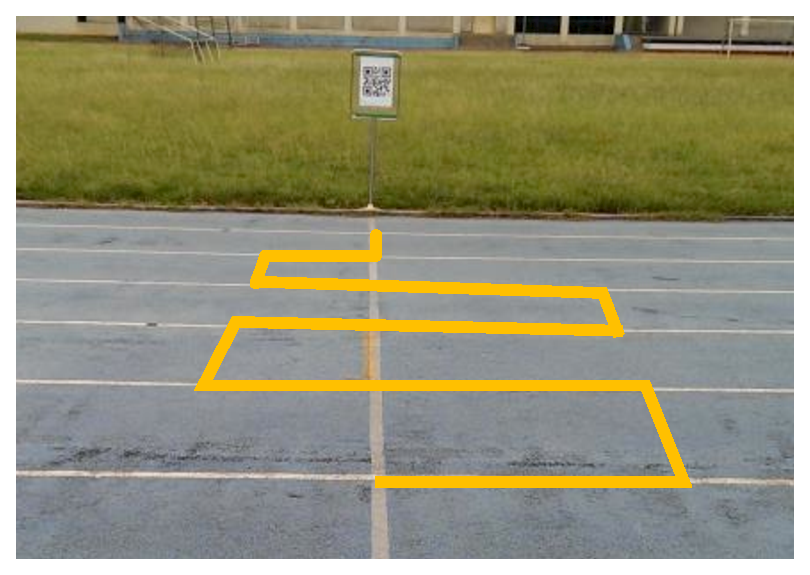
\includegraphics[width=\textwidth]{fig/small-scale-scenes.eps}
      %\vspace*{-10pt}
      \caption{Small-scale field experiment scenes.}\label{fg-small-scale-scenes}
    \end{minipage}
    \quad \quad
    \begin{minipage}[t]{0.5\textwidth}
      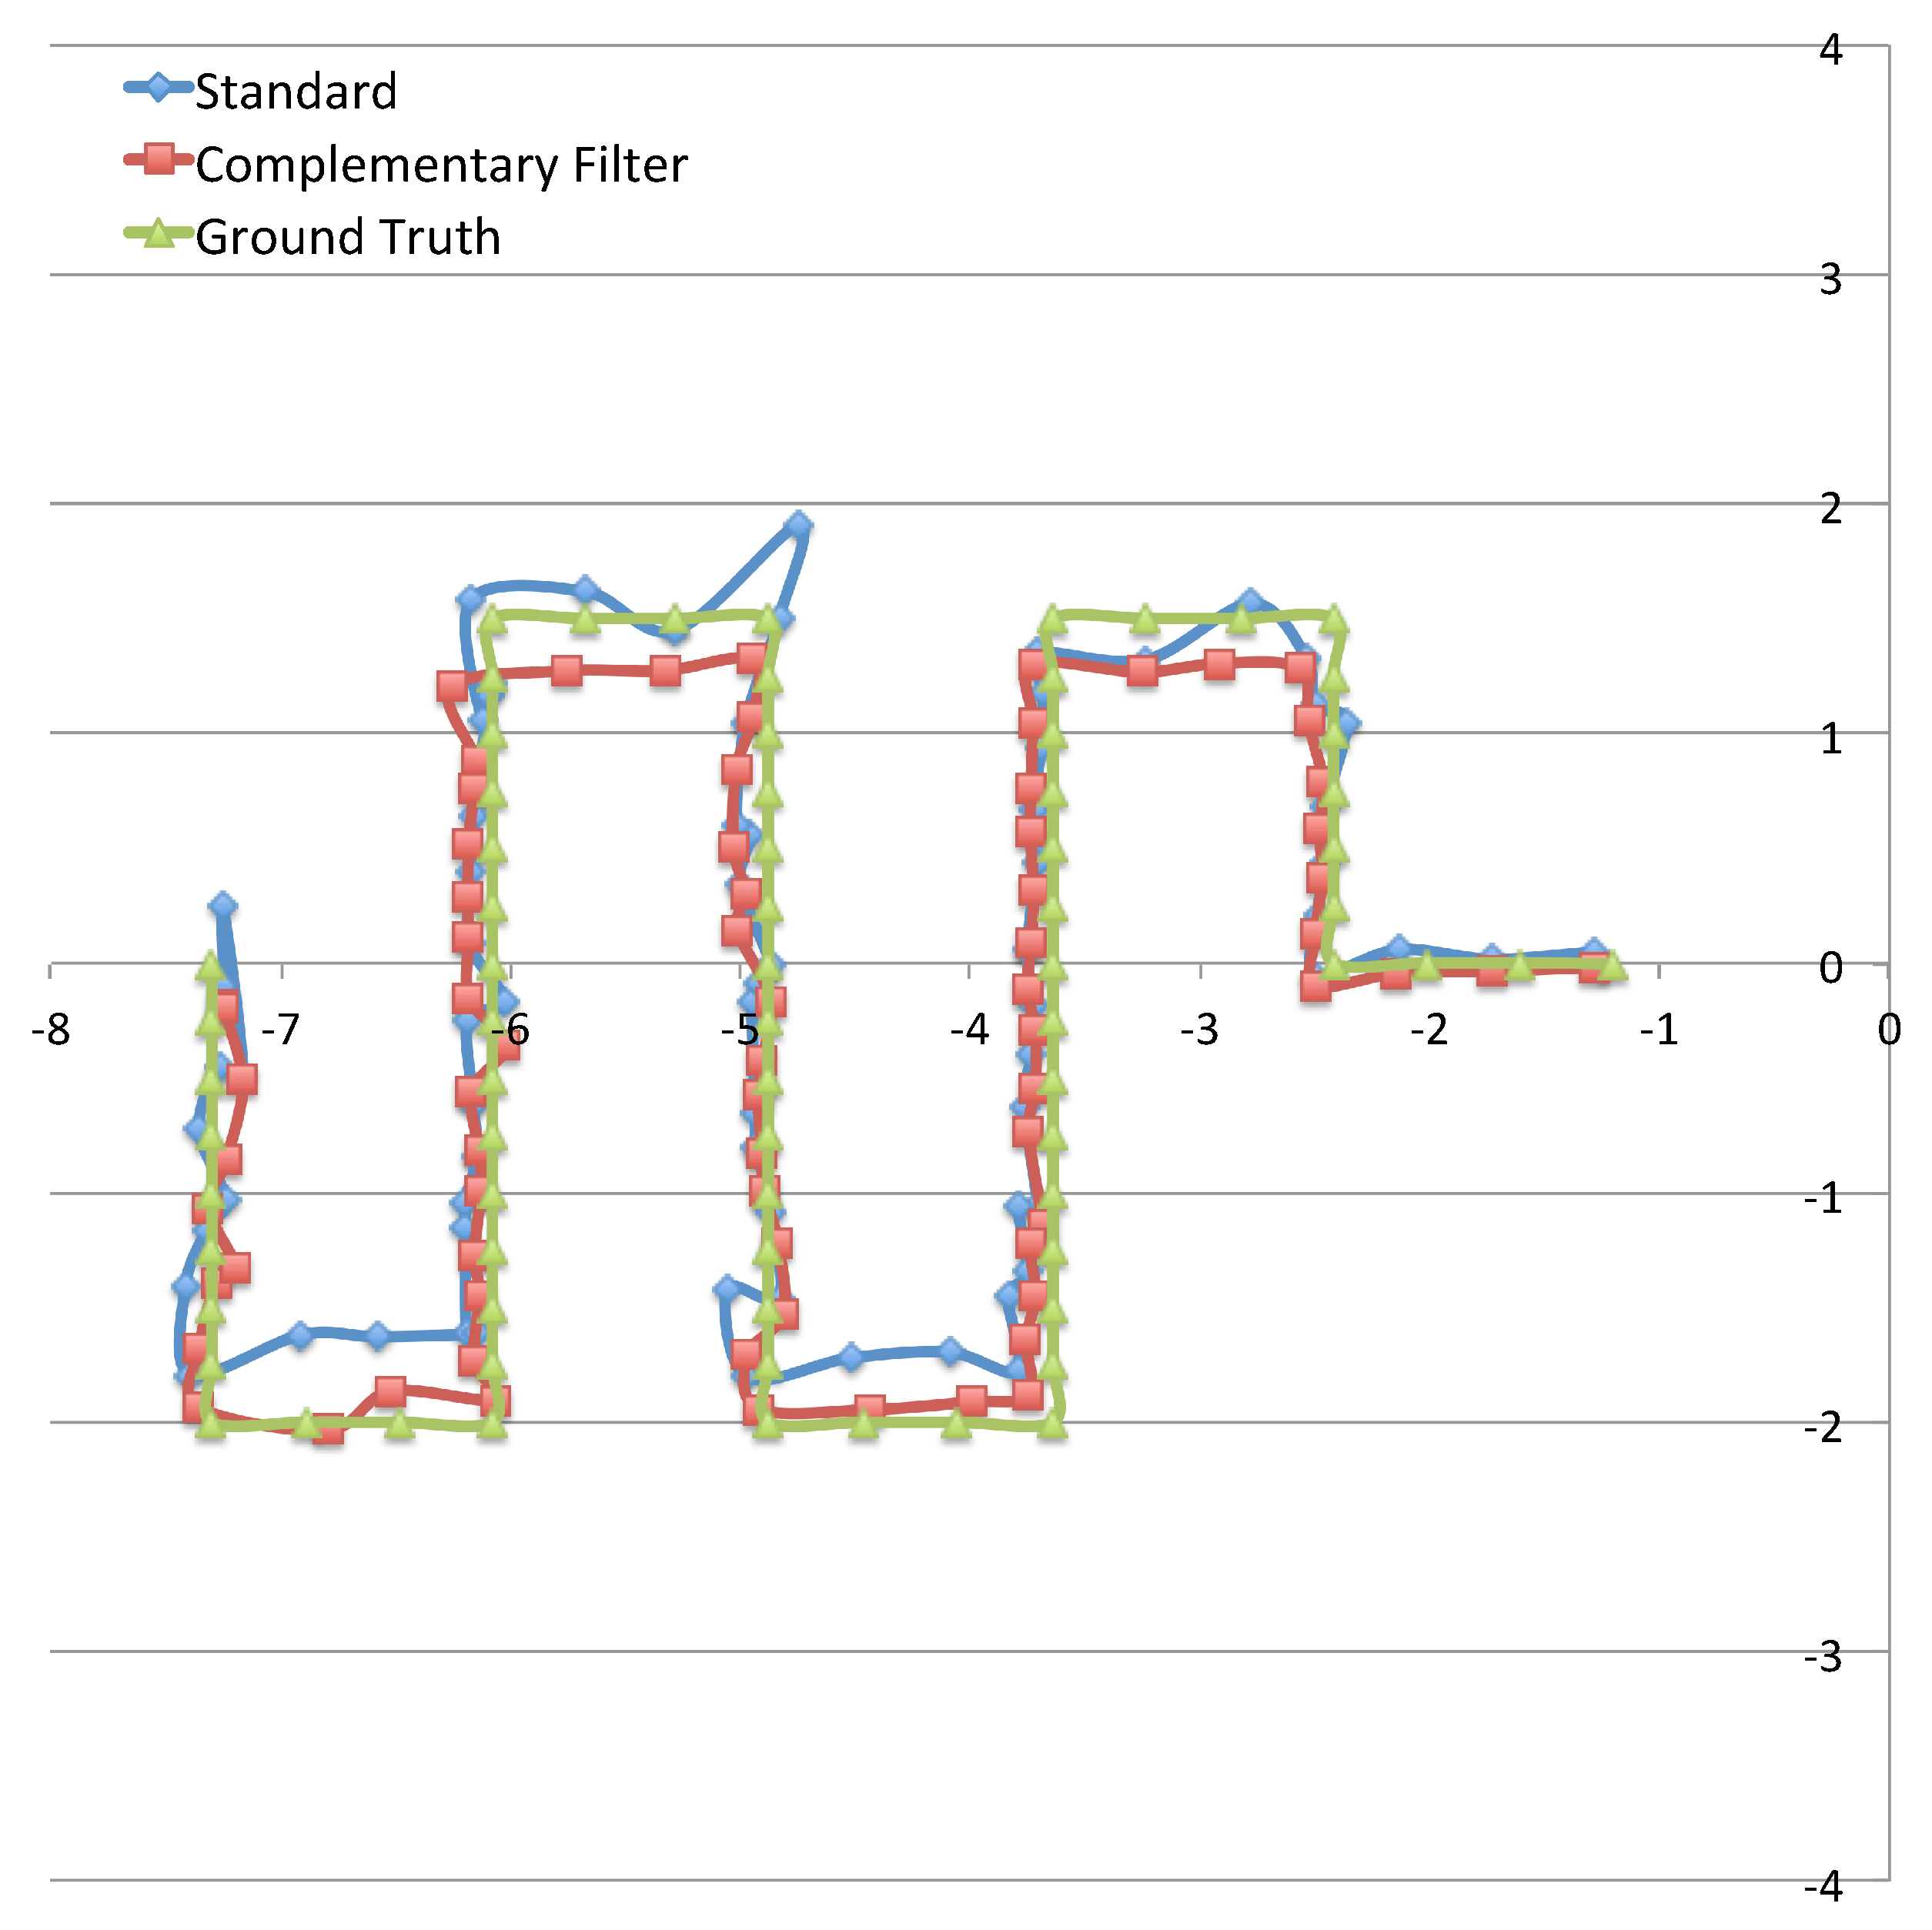
\includegraphics[width=\textwidth]{fig/small-scale-chart.eps}
      %\vspace*{-10pt}
      \caption{Small-scale field experiment log chart.}\label{fg-small-scale-chart}
    \end{minipage}
  \end{tabular}
\end{center}
\vspace{-20pt}
\end{figure*}
%%\begin{figure}
%  \centering
%  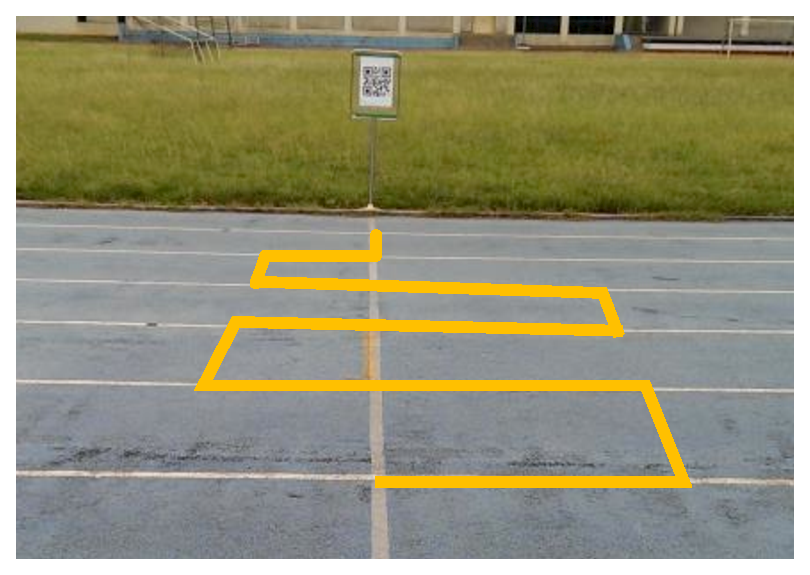
\includegraphics[width=3.3in]{fig/small-scale-scenes.eps}\\
%  \caption{Small-scale field experiment scenes.}\label{fg-small-scale-scenes}
%\end{figure}
%\begin{figure}
%  \centering
%  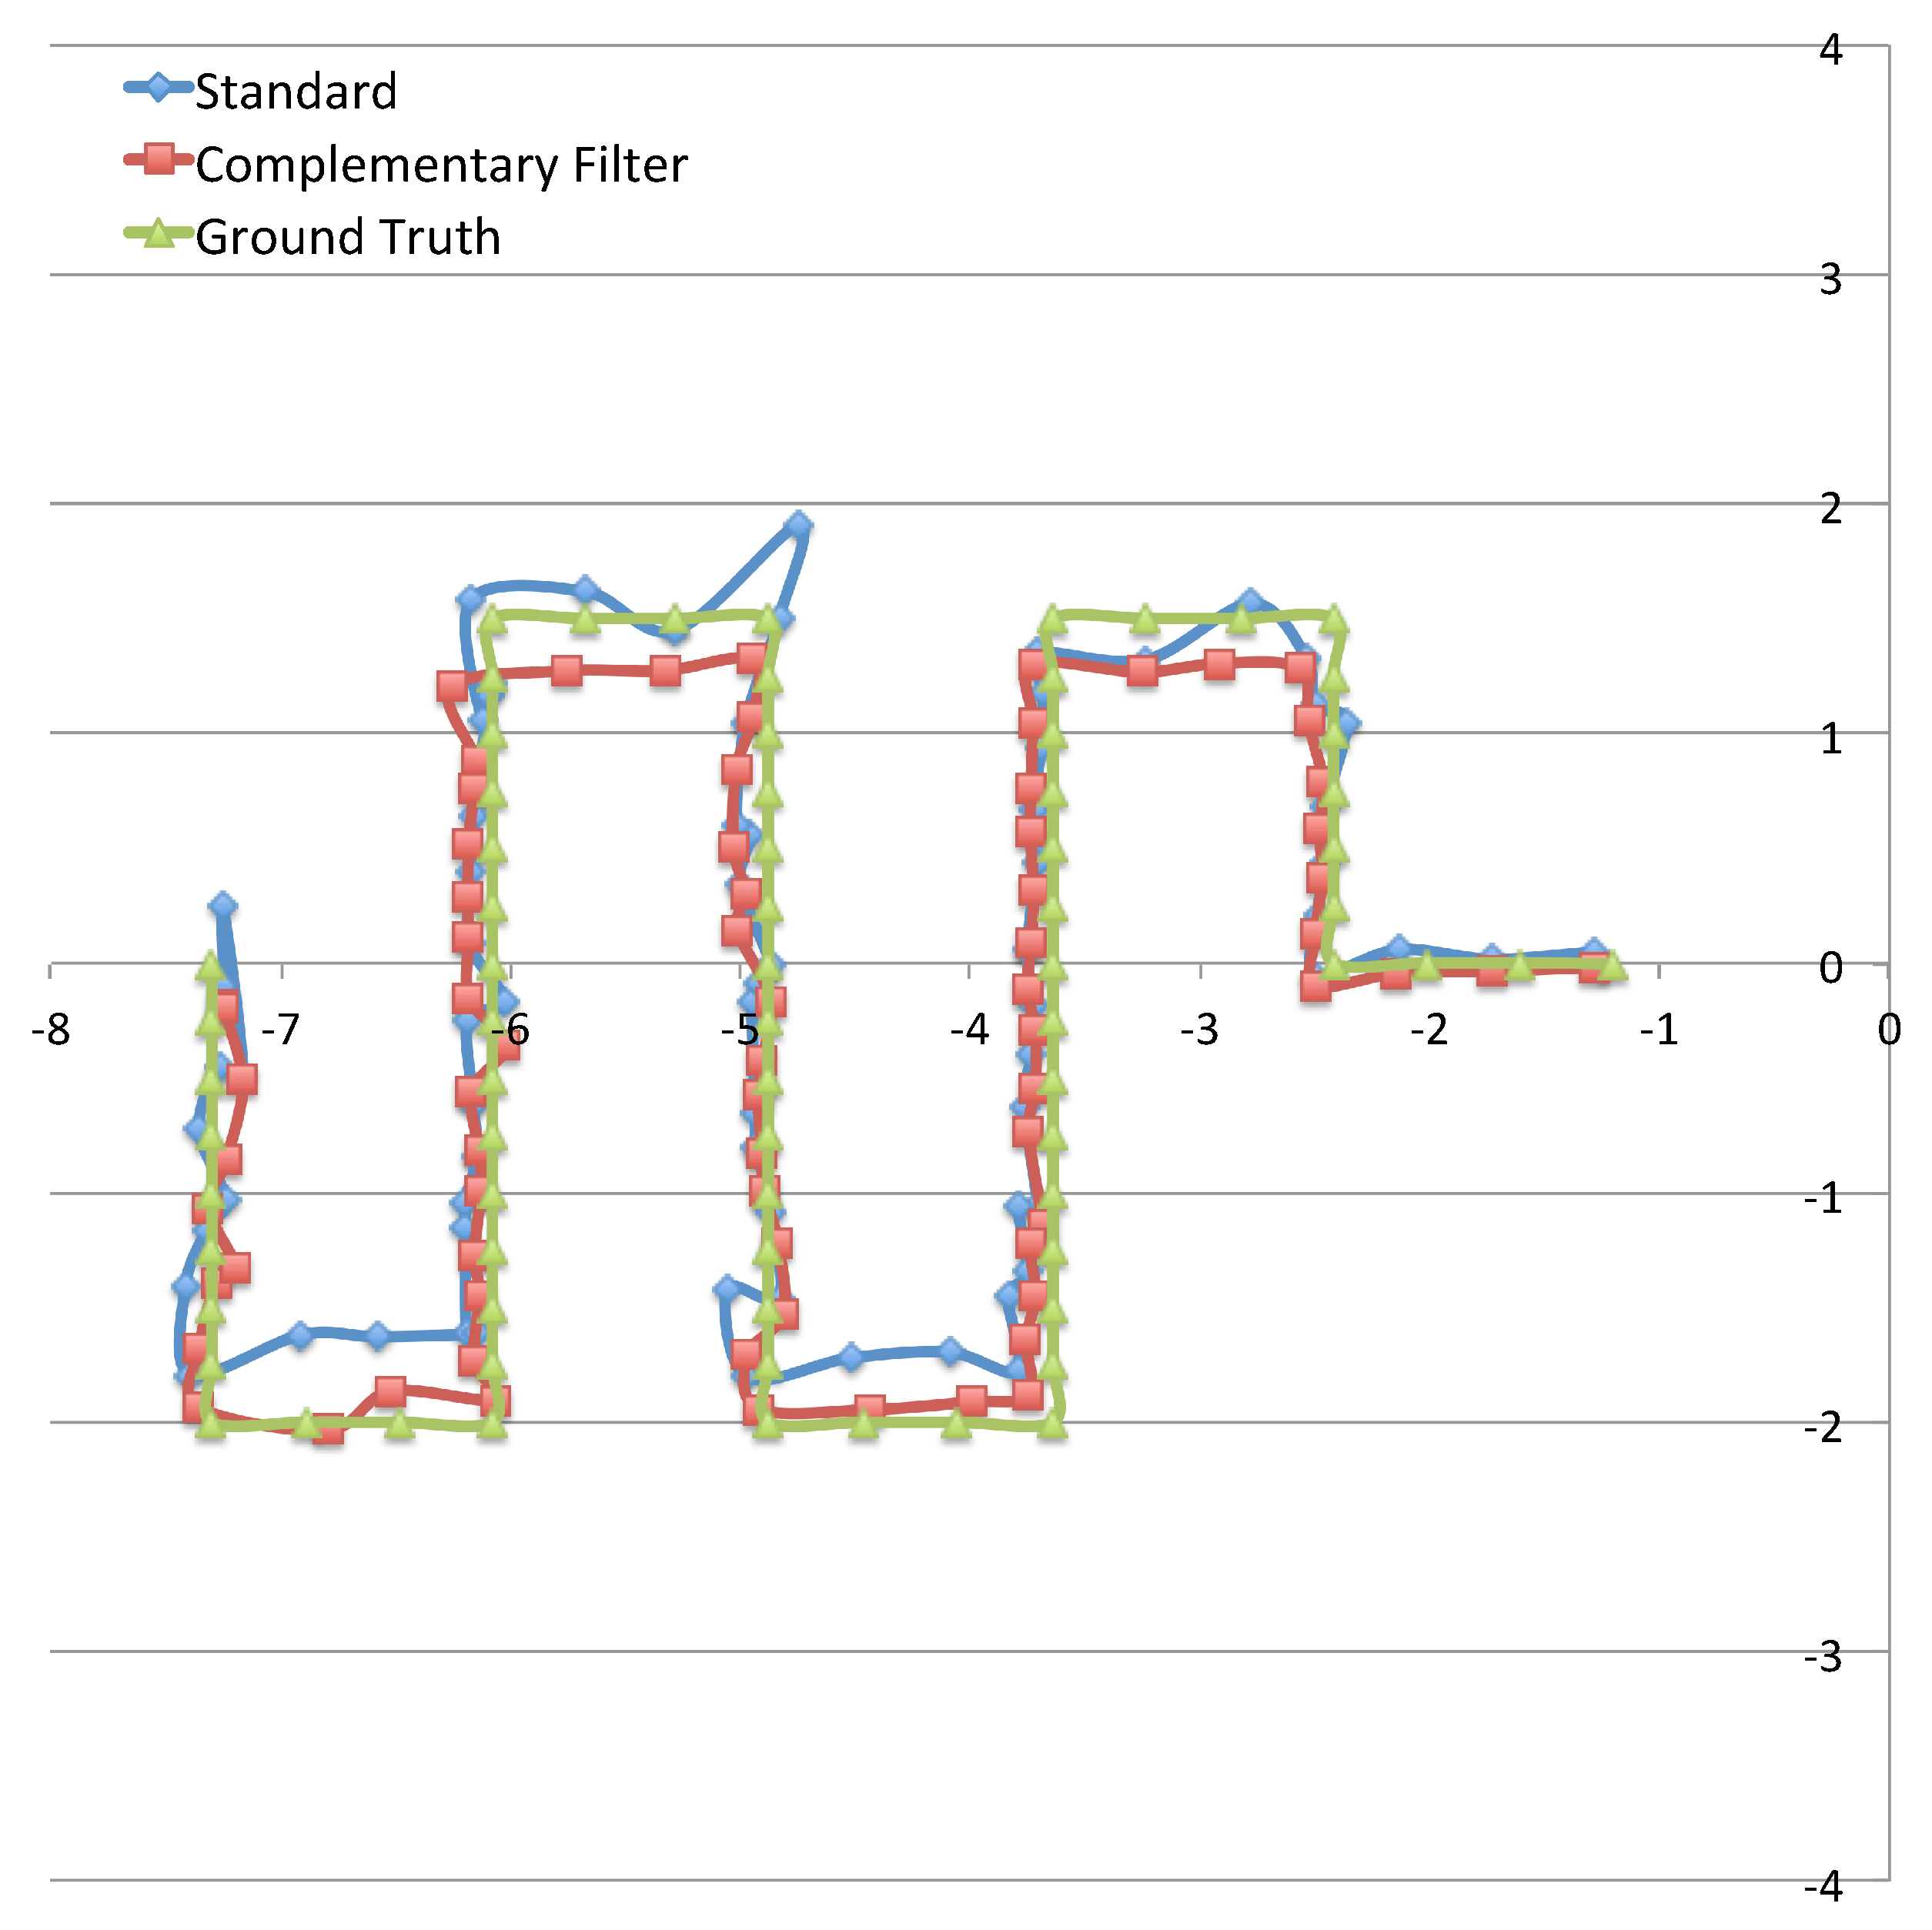
\includegraphics[width=3.3in]{fig/small-scale-chart.eps}\\
%  \caption{Small-scale field experiment log chart.}\label{fg-small-scale-chart}
%%\end{figure}
\begin{wraptable}{r}{6.5cm}
\begin{center}
\vspace{-35pt}
    \begin{tabular}{ | l | l | l |}
    \hline
    Description & Standard & Complementary \\ \hline\hline
    Max Error Distance & 0.496 meters & 0.374 meters \\ \hline
    Min Error Distance & 0.112 meters & 0.022 meters \\ \hline
    Average Error Ratio & 4.11\% & 3.61\% \\ \hline
    Standard Deviation & 0.1 meters & 0.07 meters \\ \hline
    \end{tabular}
\end{center}
\vspace{-15pt}
\caption{Small-scale field experiment statistic results.}\label{tb-small-scale-analysis}
\vspace{-15pt}
\end{wraptable} 
The results of the small-scale field experiments demonstrate that the error rate of the positioning is lower than 5\%, and the maximal error distance is smaller than 0.5 meters. This results indicate that the system has a high precision for positioning in situations such as in a classroom, a conference room, or a living room.
\subsection{Median-scale field experiments}
For median-scale field experiments, we choose a 16m x 35m plaza as the experiment environment. The MRP is a QR code on a poster of the size 54.3cm x 54.2cm, as can be seen in Figure~\ref{fg-median-scale-scenes}. Similar to the small-scale experiments, the collected data includes standard e-compass and complementary filter results. In addition, we also collect the GPS results obtained from a \emph{Garmin Dakota 20} navigation device. The experiment and the statistic results are shown in Figure~\ref{fg-median-scale-chart} and Table~\ref{tb-median-scale-analysis}, respectively.\\
\begin{figure*}[th!]
\begin{center}
 \begin{tabular}[t]{ccc}
    \begin{minipage}[t]{0.5\textwidth}
      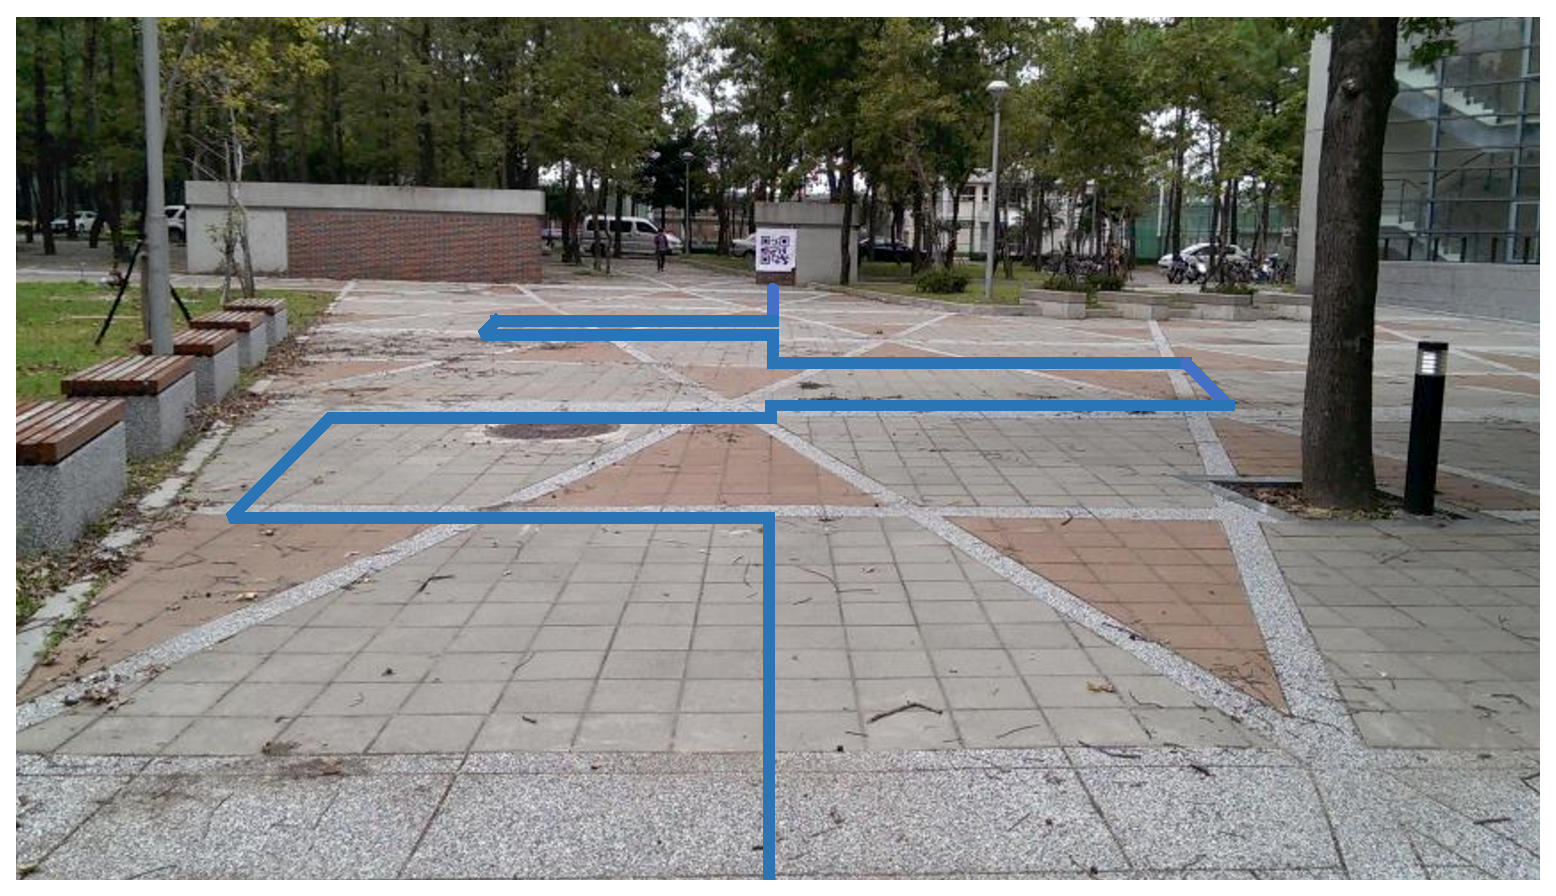
\includegraphics[width=\textwidth]{fig/median-scale-scenes.eps}
      %\vspace*{-10pt}
      \caption{Median-scale field experiment scenes.}\label{fg-median-scale-scenes}
    \end{minipage}
    \quad \quad
    \begin{minipage}[t]{0.3\textwidth}
      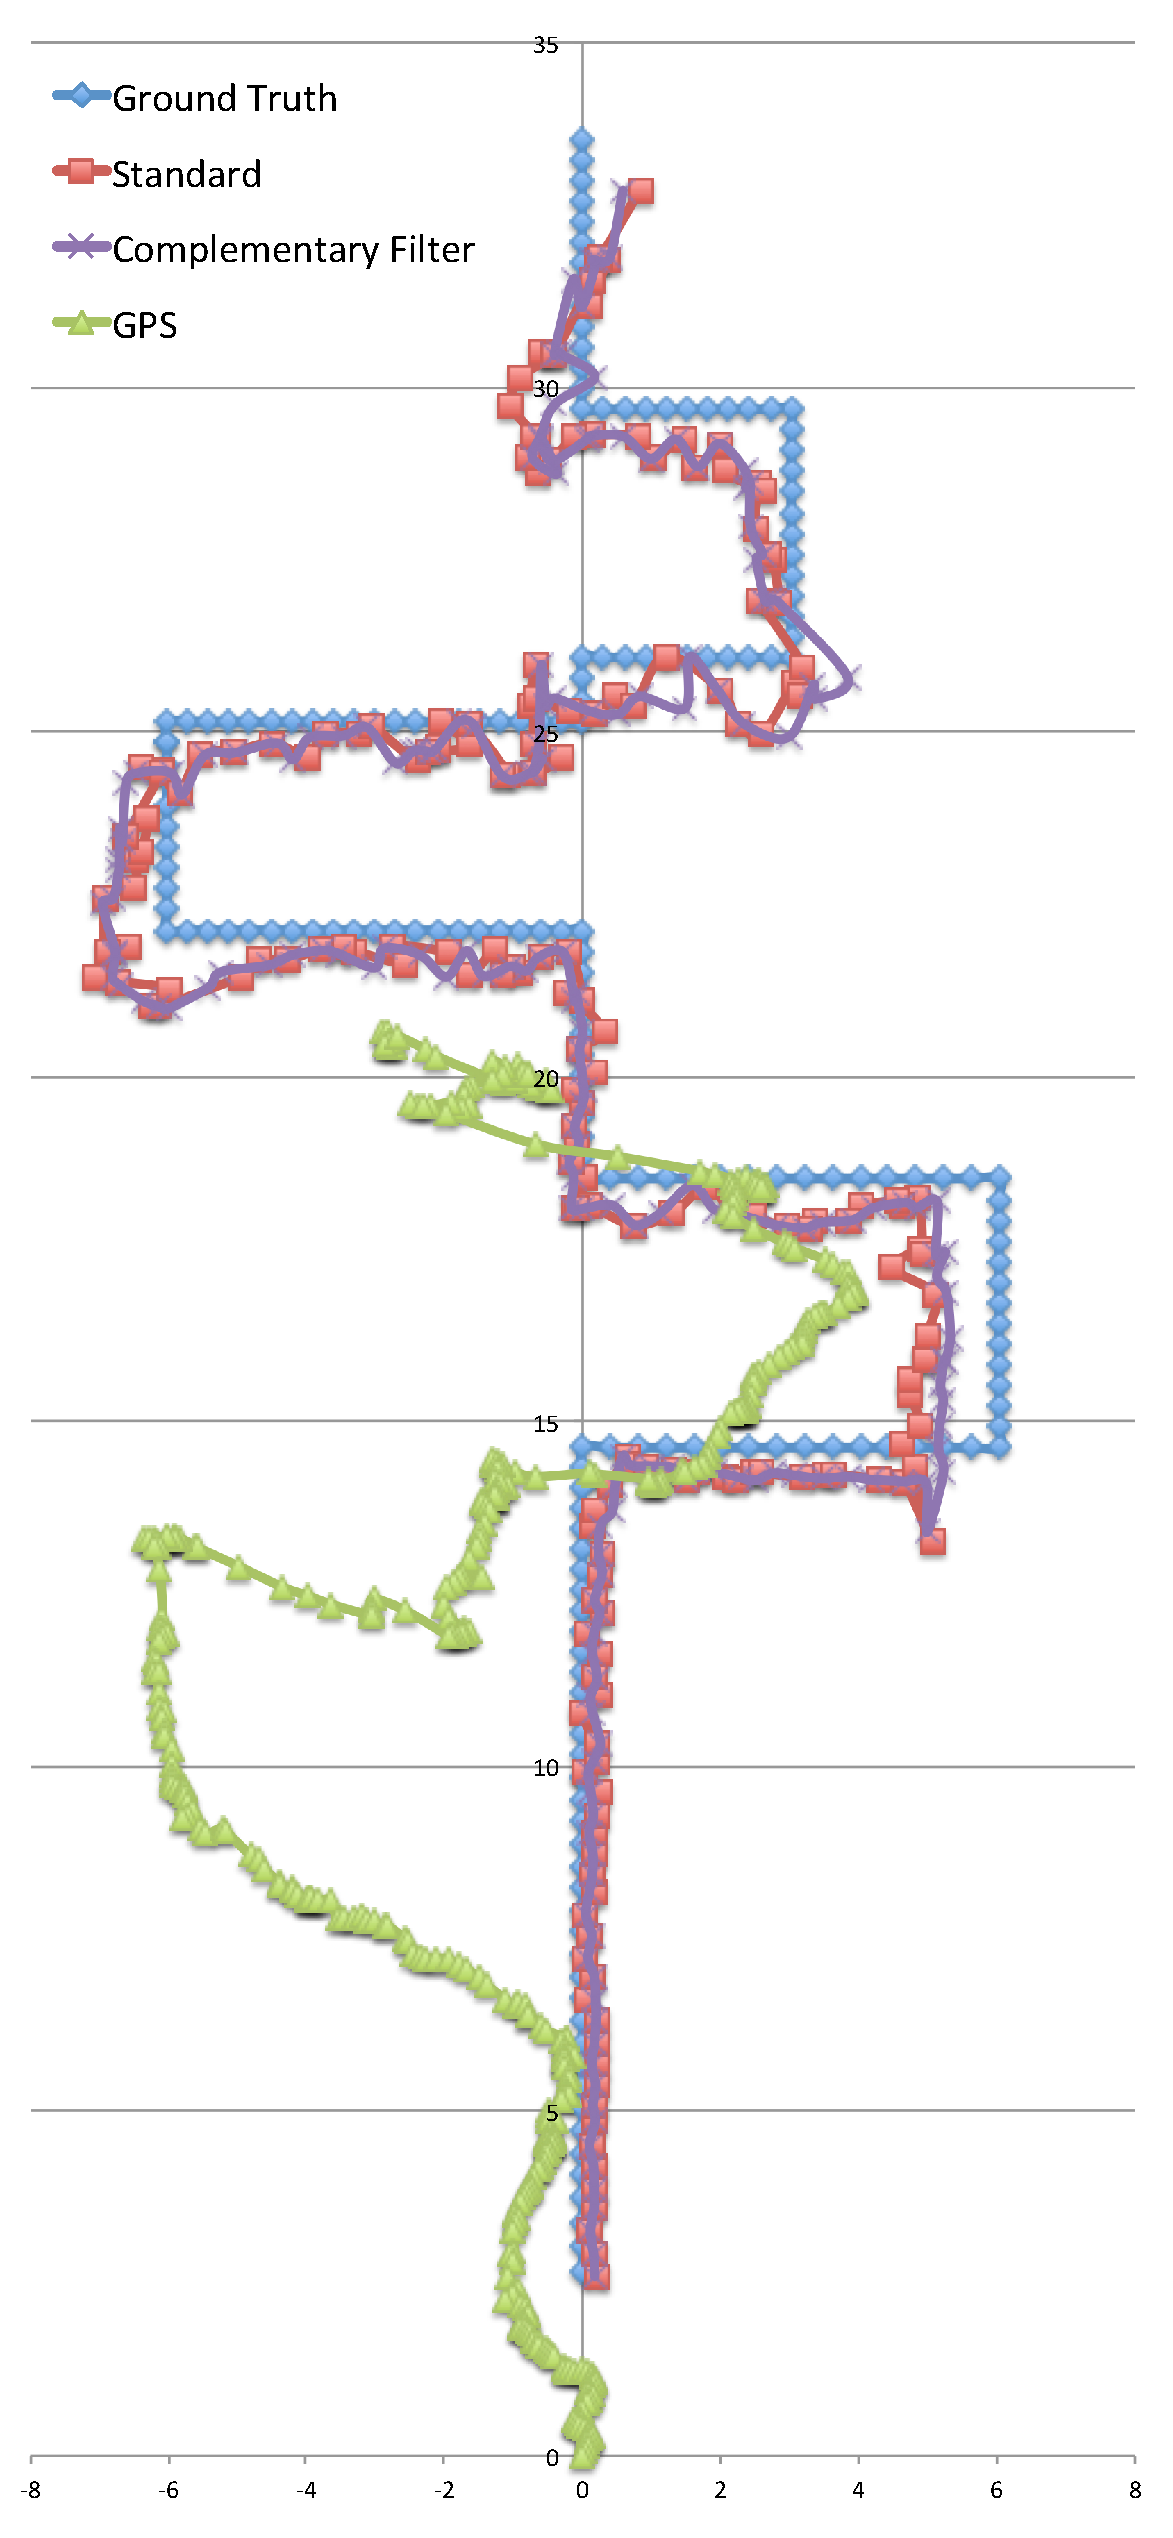
\includegraphics[width=\textwidth]{fig/median-scale-chart.eps}
      %\vspace*{-10pt}
      \caption{Median-scale field experiment results.}\label{fg-median-scale-chart}
    \end{minipage}
  \end{tabular}
\end{center}
\end{figure*}

\begin{wraptable}{r}{6.5cm}
\begin{center}
\vspace{-10pt}
    \begin{tabular}{ | l | l | l |}
    \hline
    Description & Standard & Complementary \\ \hline\hline
    Max Error Distance & 1.91 meters & 1.85 meters \\ \hline
    Min Error Distance & 0.07 meters & 0.09 meters \\ \hline
    Average Error Ratio & 4.49\% & 4.18\% \\ \hline
    Standard Deviation & 0.4 meters & 0.36 meters \\ \hline
    \end{tabular}
\end{center}
\vspace{-15pt}
\caption{Median-scale field experiment statistic results.}\label{tb-median-scale-analysis}
\vspace{-15pt}
\end{wraptable} 
The results of the median-scale field experiments demonstrate that the system has a much higher accuracy rate for positioning than the conventional GPS. For instance, the maximal error distance of our system is shorter than 2 meters, which is smaller than even the error of the assisted GPS. This results indicate that our system are suitable for indoor navigation in a shopping mall or a large exhibit hall.

\subsection{Large-scale field experiments}
\begin{wrapfigure}{r}{2in}
  \vspace{-20pt}
  \centering
  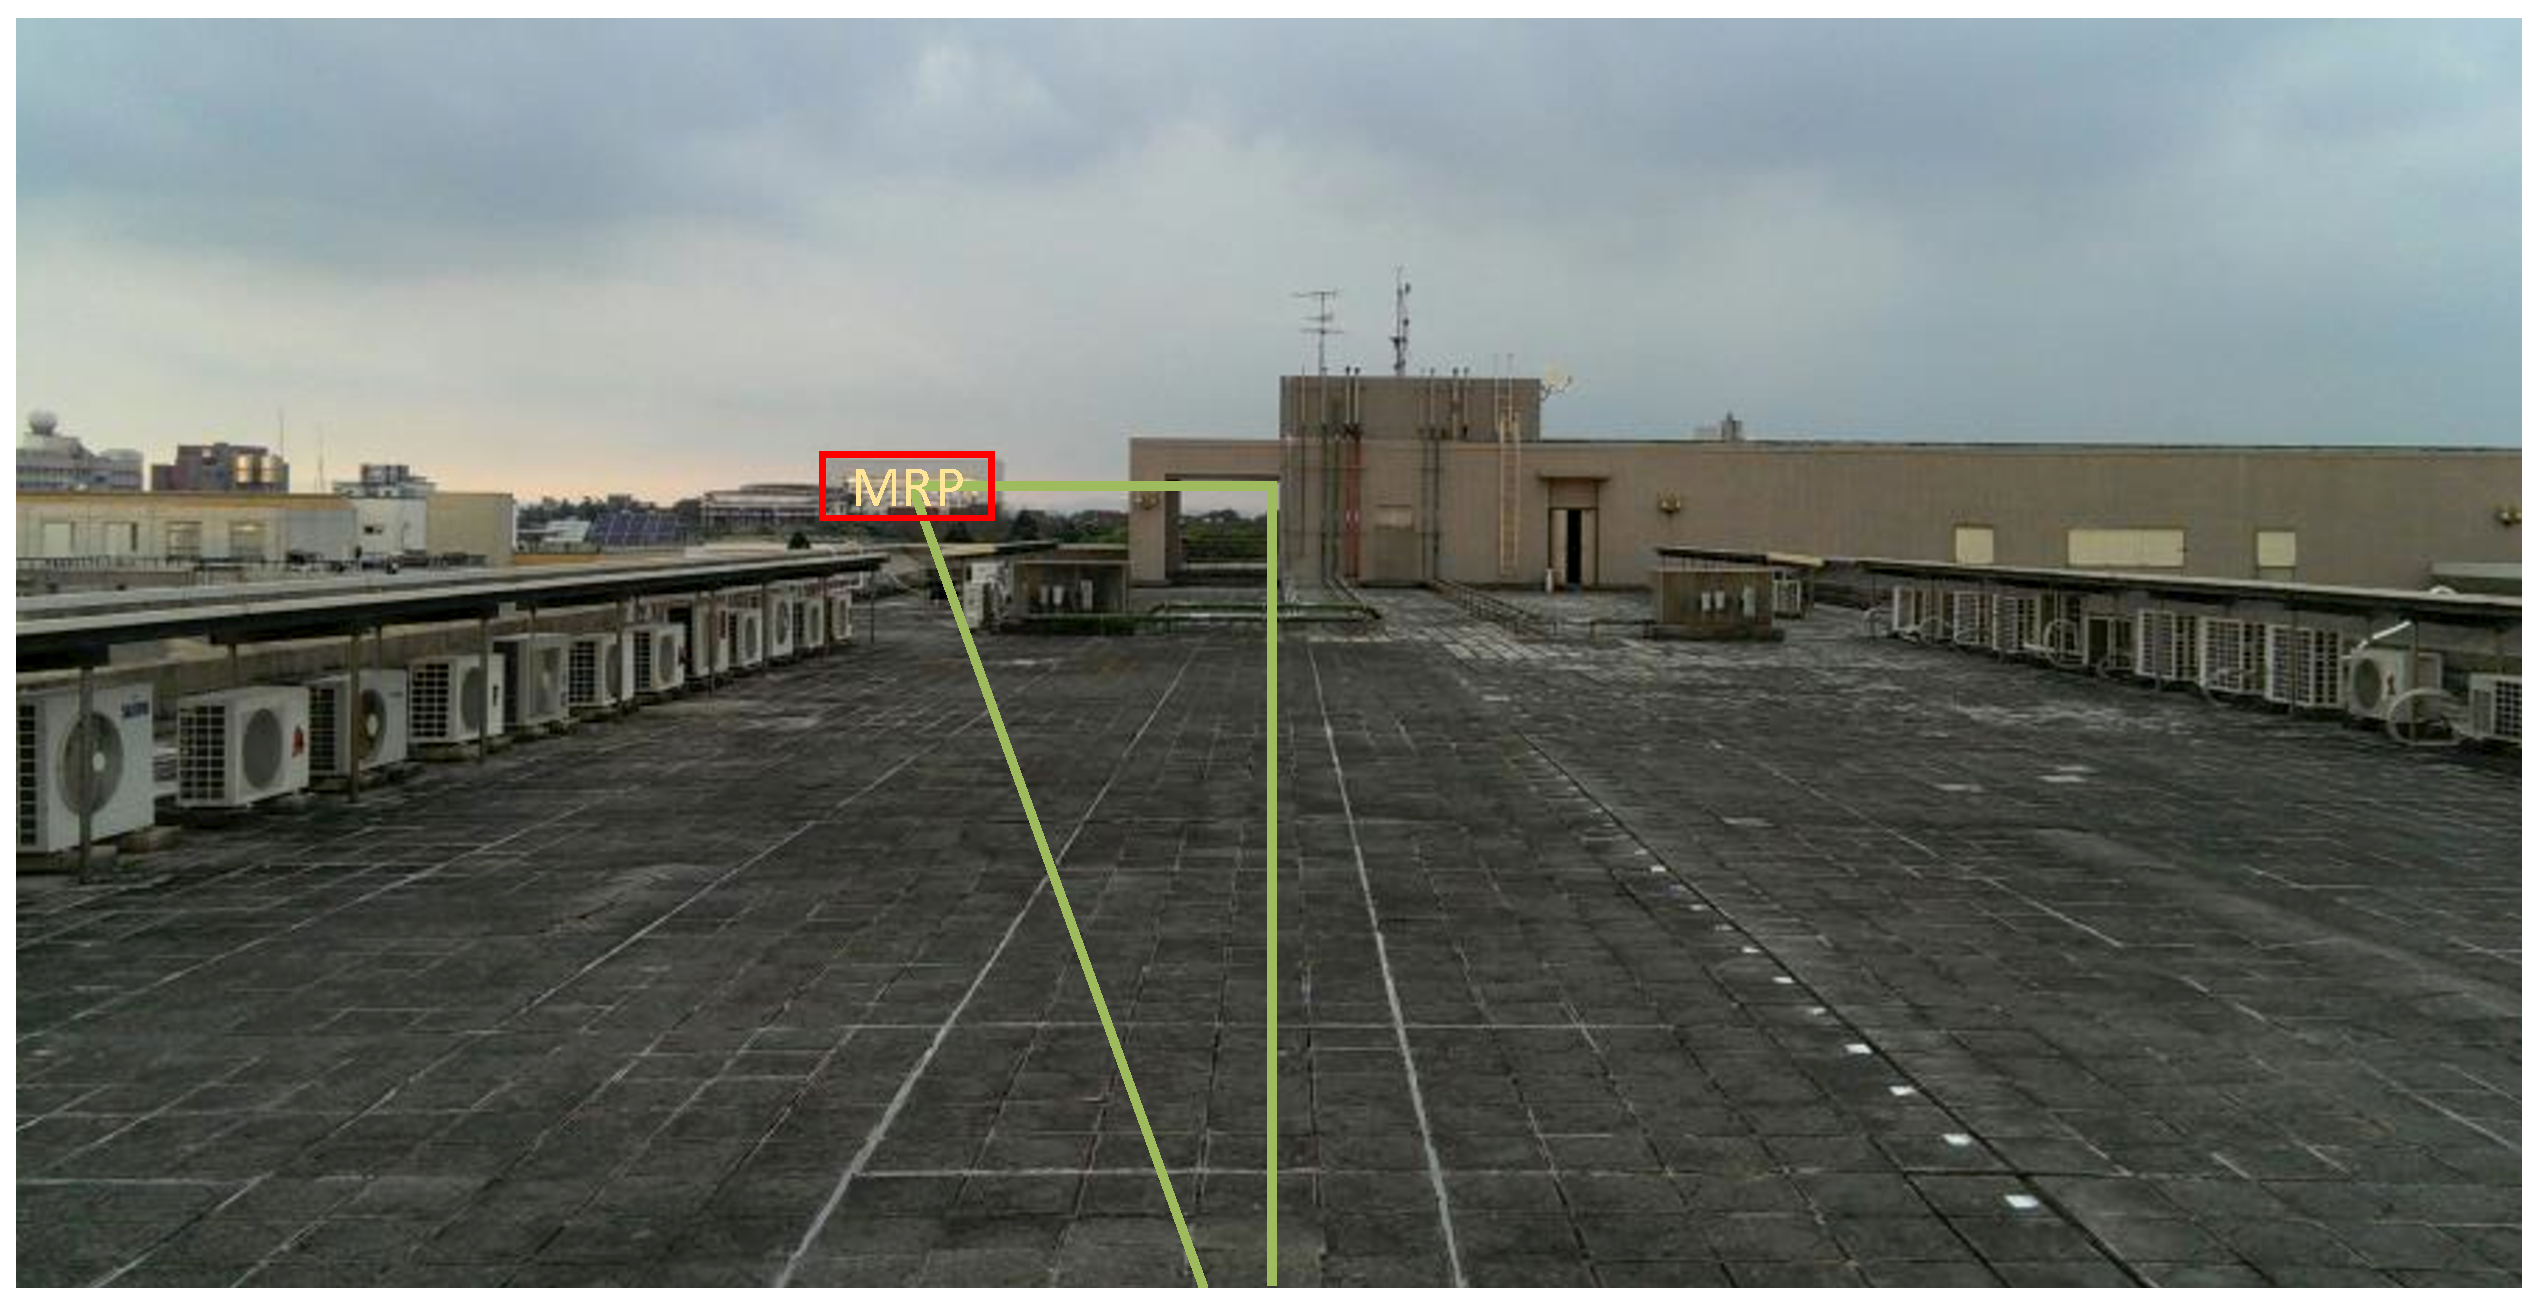
\includegraphics[width=3.3in]{fig/large-scale-scenes.eps}\\
  \vspace{-10pt}
  \caption{Large-scale field experiment scenes in National Central University.}\label{fg-large-scale-scenes}
  \vspace{-90pt}
\end{wrapfigure}
For large-scale field experiments, we choose the NCU Main Library Building as the MRP. We stand on the rooftop of the Engineering Building 5 facing the MRP to obtain our position, as illustrated in Figure~\ref{fg-large-scale-scenes}. The range between the MRP and us is around 800 meters.

\begin{table*}[th!]
\begin{center}
 \begin{tabular}[t]{ccc}
    \begin{minipage}[t]{0.6\textwidth}
    \begin{tabular}{ | l | l | l | l |}
    \hline
    \multicolumn{2}{ |c| }{Standard} & \multicolumn{2}{ c| }{Complementary} \\ \hline
    Error Distance & Error Ratio & Error Distance & Error Ratio \\ \hline
    \hline
    55.94779483 & 7.63\% & 41.01243255 & 5.59\% \\ \hline
    23.760599 & 3.24\% & 30.46624108 & 4.15\% \\ \hline
    55.33866059 & 7.53\% & 32.29396614 & 4.40\% \\ \hline
    16.77831869 & 2.29\% & 30.22630963 & 4.12\% \\ \hline
    30.18733363 & 4.11\% & 29.07574148 & 3.96\% \\ \hline
    18.36331176 & 2.50\% & 13.21252122 & 1.80\% \\ \hline
    22.71171715 & 3.10\% & 17.99106596 & 2.45\% \\ \hline
    17.22804678 & 2.35\% & 14.44225332 & 1.97\% \\ \hline
    29.55978553 & 4.03\% & 14.68165469 & 2.00\% \\ \hline
    \end{tabular}
    \caption{Large-scale field experiment error ratio.}\label{tb-large-scale-values}
    \end{minipage}
    \quad \quad
    \begin{minipage}[t]{0.6\textwidth}
    \begin{tabular}{ | l | l | l | l |}
    \hline
    Description & Standard & Complementary \\ \hline
    \hline
    Max Error Distance & 55.95 meters & 41.01 meters \\ \hline
    Min Error Distance & 16.78 meters & 13.21 meters \\ \hline
    Average Error Ratio & 4.09\% & 3.3\% \\ \hline
    Standard Deviation & 15.33 meters & 993 meters \\ \hline
    \end{tabular}
    \caption{Large-scale field experiment statistic results.}\label{tb-large-scale-analysis}
    \end{minipage}
  \end{tabular}
\end{center}
\end{table*}

The experiment results are shown in Figure~\ref{large-scale-campus-map} and Figure~\ref{large-scale-building5-map}. In the figures, the main library is denoted by an icon and our true position (obtained by GPS) is denoted by a red flag. Each blue circle indicates a result of the standard method, and each red circle is a result of the complementary filter method. The statistic results are shown in Table~\ref{tb-large-scale-values} and Table~\ref{tb-large-scale-analysis}.\\

The results of the large-scale field experiments indicate that although the percentage of the error of our system is low (less than 5\% in most cases), the absolute error of our system can be quite large when the MRP is far away from the camera. For instance, the maximal error distance is about 40 meters in our large-scale experiments, even when the complementary filter is applied. For applications such as virtual augmentations and location-based services, this accuracy is acceptable. However, for applications that require a high precision, our system may not be suitable. 
\begin{figure*}[th!]
\begin{center}
 \begin{tabular}[t]{ccc}
    \begin{minipage}[t]{0.5\textwidth}
      \includegraphics[width=\textwidth]{fig/large-scale-campus-map.eps}
      %\vspace*{-10pt}
      \caption{Campus map to large-scale field experiment results.}\label{large-scale-campus-map}
    \end{minipage}
    \quad \quad
    \begin{minipage}[t]{0.5\textwidth}
      \includegraphics[width=\textwidth]{fig/large-scale-building5-map.eps}
      %\vspace*{-10pt}
      \caption{Zoom in Engineering Building 5 map to large-scale field experiment results.}\label{large-scale-building5-map}
    \end{minipage}
  \end{tabular}
\end{center}
\end{figure*}